\chapter{Related Work}
\label{ch:state_of_the_art}

The ocean surface is an intricate phenomenon which owes its complexity in large part
to its highly dynamic nature. Be it a quiet sea or an agitated one, small turbulent waves
or huge breaking ones, the underlying mechanisms are manifold and act on different scales.
Oceanographic research distinguishes between the deep ocean e.g. water far from the coast,
and shallow water e.g. water close to the shore.  The former is governed by the interaction
of wind and gravity at the interface between air and water, whereas the latter is
characterized by waves breaking near the shore.

To date, computer graphics employs several ocean wave models, which can be separated into
three families: parametric description, spectral description, computational fluid dynamics.


Simulation, Animation

Parametric model
Spectral Models
Computational Fluid Dynamics
Navier Stokes

Rendering

Particles
Reflection
Refraction
Foam, Sprays

Parametric\\
Perlin - An Image Synthesizer \cite{Perlin:1985}\\
Nelson Max - Vectorized Procedural Models for Natural Terrain: Waves and Islands in the Sunset \cite{Max:1981}\\
Peachey - Modeling Waves and Surf \cite{Peachey:1986}\\
Fournier - A simple model of ocean waves \cite{Fournier:1986}\\
Ts'o - Modeling and rendering waves: Wave-tracing using beta-splines and reflective and refractive texture mapping \cite{Ts'o:1987}\\Hinsinger - Interactive Animation of Ocean Waves \cite{Hinsinger:2002}\\

Spectral\\
Mastin - Fourier Synthesis of Ocean Scenes \cite{Mastin:1987}\\
Tessendorf - Simulating Ocean Water \cite{course:simulatingocean}\\
Premoze - Rendering Natural Waters \cite{Premoze:2000} \\

Hybrid\\
Thon - Ocean waves synthesis using a spectrum based turbulence function \cite{thon:2000}\\
Lee - Real-Time Simulation of Surface Gravity Ocean Waves Based on the TMA Spectrum\cite{lee:2007}\\


\begin{figure}
\centering
 \subtop
 {
  \includegraphics[scale=0.45]{figures/ocean300_5.jpg}
 }
 \hfill
 \subtop
 {
  \includegraphics[scale=0.45]{figures/ocean_storm300.jpg}
 }
\caption{The late afternoon sun illuminating the ocean surface. Source: NOAA~\cite{misc:noaa}}
\end{figure}

\begin{figure}
 \centering
 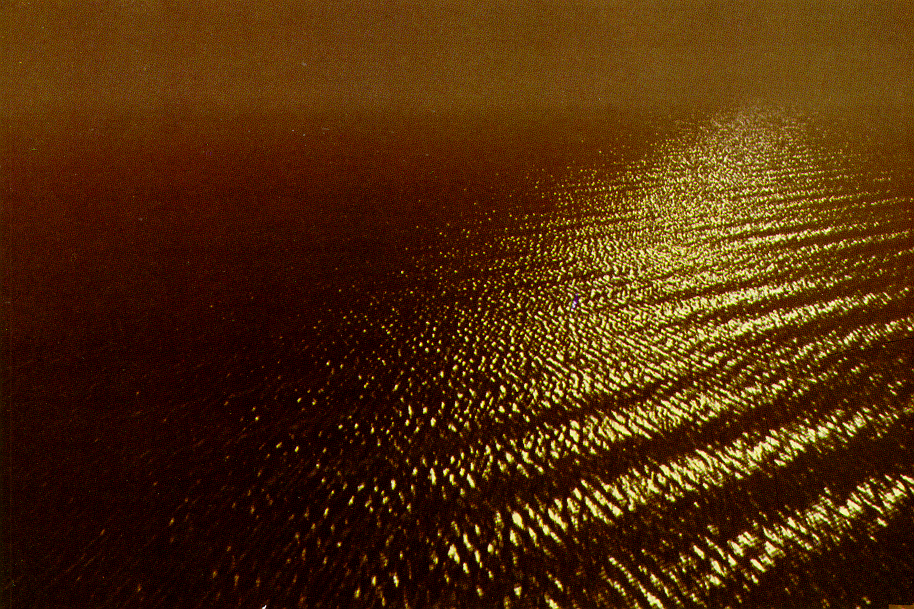
\includegraphics[scale=0.25]{figures/An_Image_Synthesizer_-_Perlin_1985-021.png}
 \caption{Perlin 1985}
\end{figure}

\begin{figure}
 \centering
 \subtop
 {
  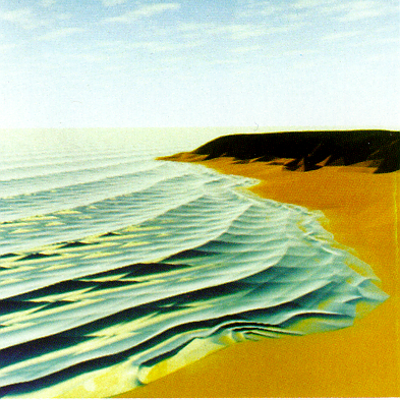
\includegraphics[scale=0.25]{figures/Modeling_Waves_and_Surf_-_Peachey_1986-009.png}
 }
 \hfill
 \subtop
 {
  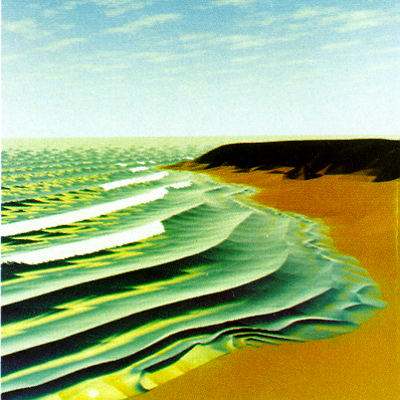
\includegraphics[scale=0.25]{figures/Modeling_Waves_and_Surf_-_Peachey_1986-010.png}
 }
 \hfill
 \subtop
 {
  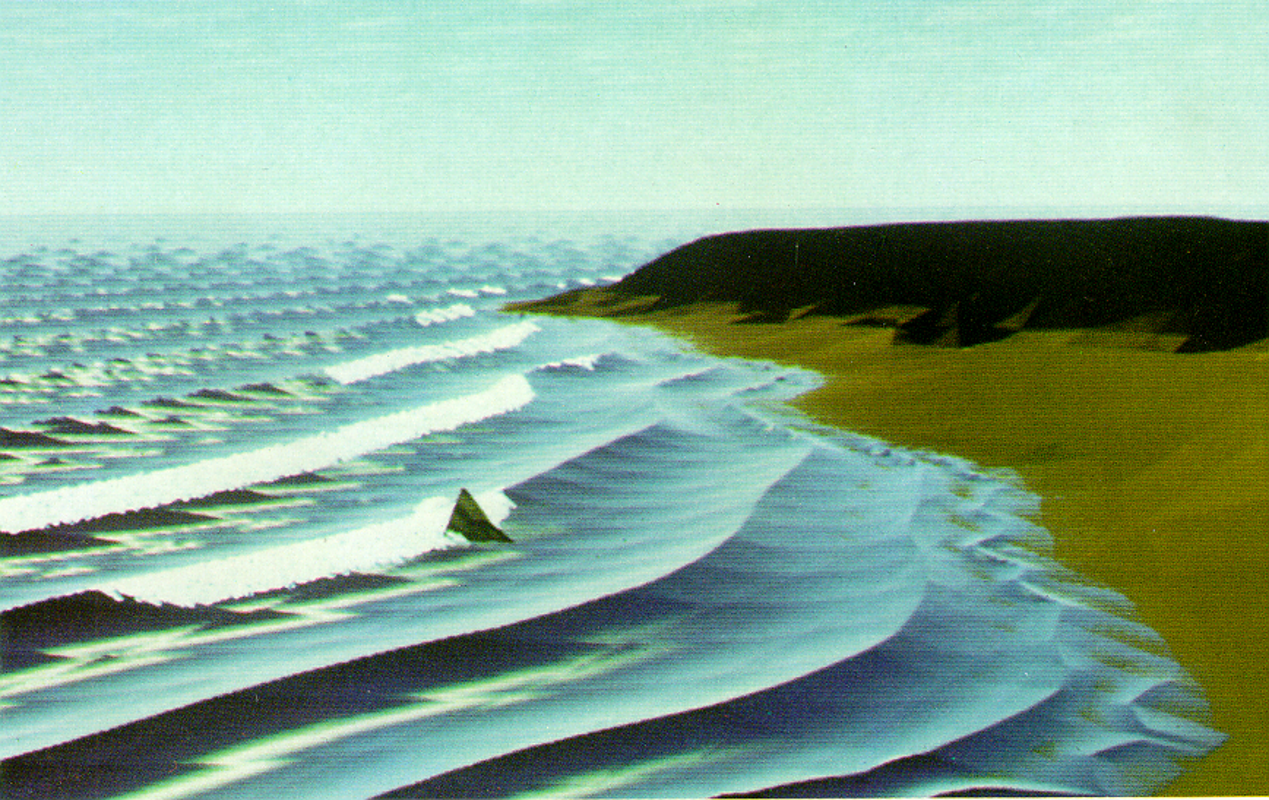
\includegraphics[scale=0.125]{figures/Modeling_Waves_and_Surf_-_Peachey_1986-012.png}
 }
 \caption{Peachey 1986}
\end{figure}

\begin{figure}
 \centering
 \subtop
 {
  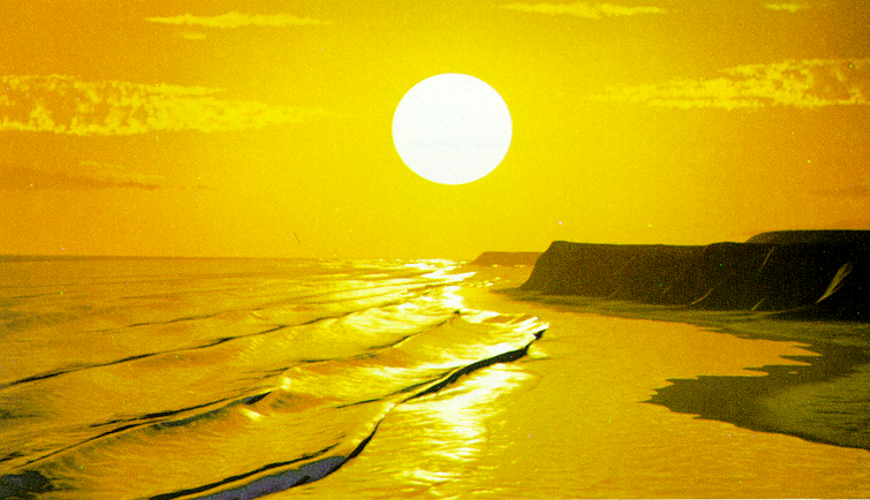
\includegraphics[scale=0.225]{figures/A_Simple_Model_of_Ocean_Waves_-_Fournier_1986-008.png}
 }
 \hfill
 \subtop
 {
  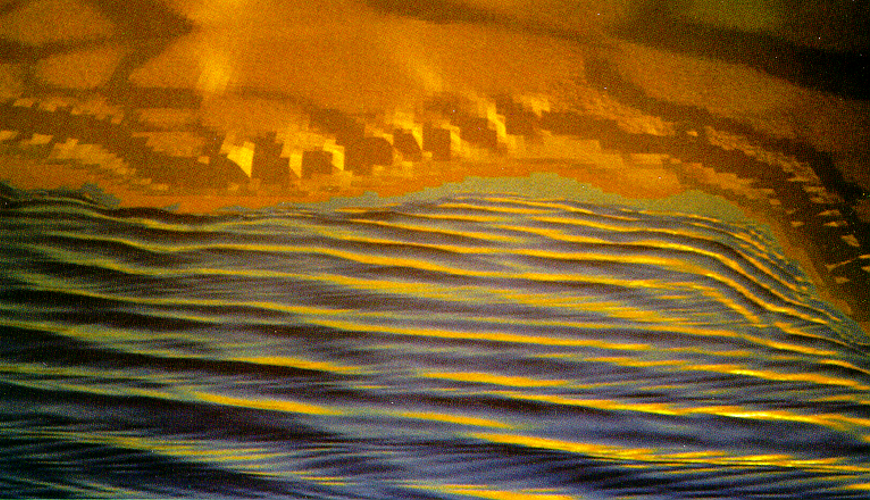
\includegraphics[scale=0.225]{figures/A_Simple_Model_of_Ocean_Waves_-_Fournier_1986-010.png}
 }
 \subtop
 {
  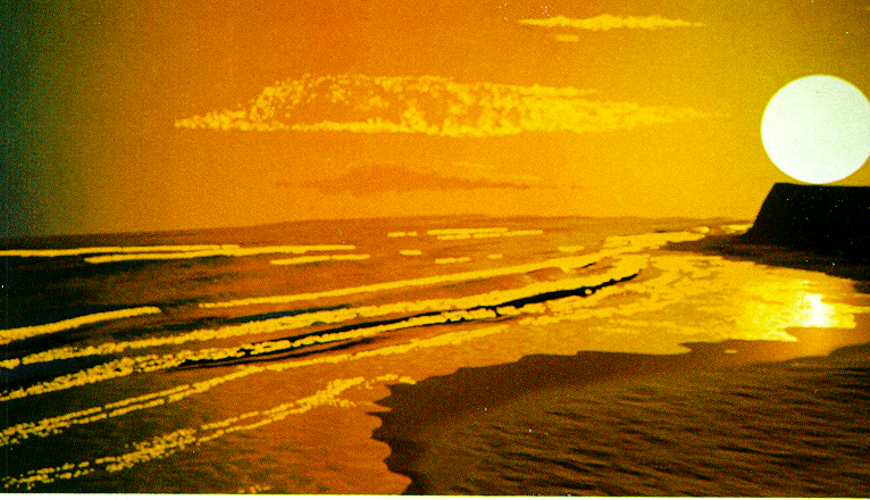
\includegraphics[scale=0.225]{figures/A_Simple_Model_of_Ocean_Waves_-_Fournier_1986-011.png}
 }
 \hfill
 \subtop
 {
  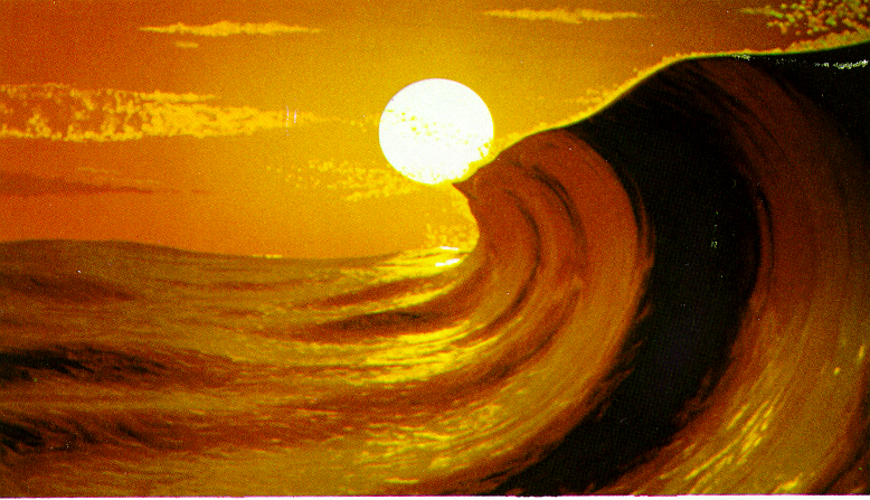
\includegraphics[scale=0.225]{figures/A_Simple_Model_of_Ocean_Waves_-_Fournier_1986-013.png}
	}
 \caption{Fournier 1986}
\end{figure}

\begin{figure}
 \centering
 \subtop
 {
  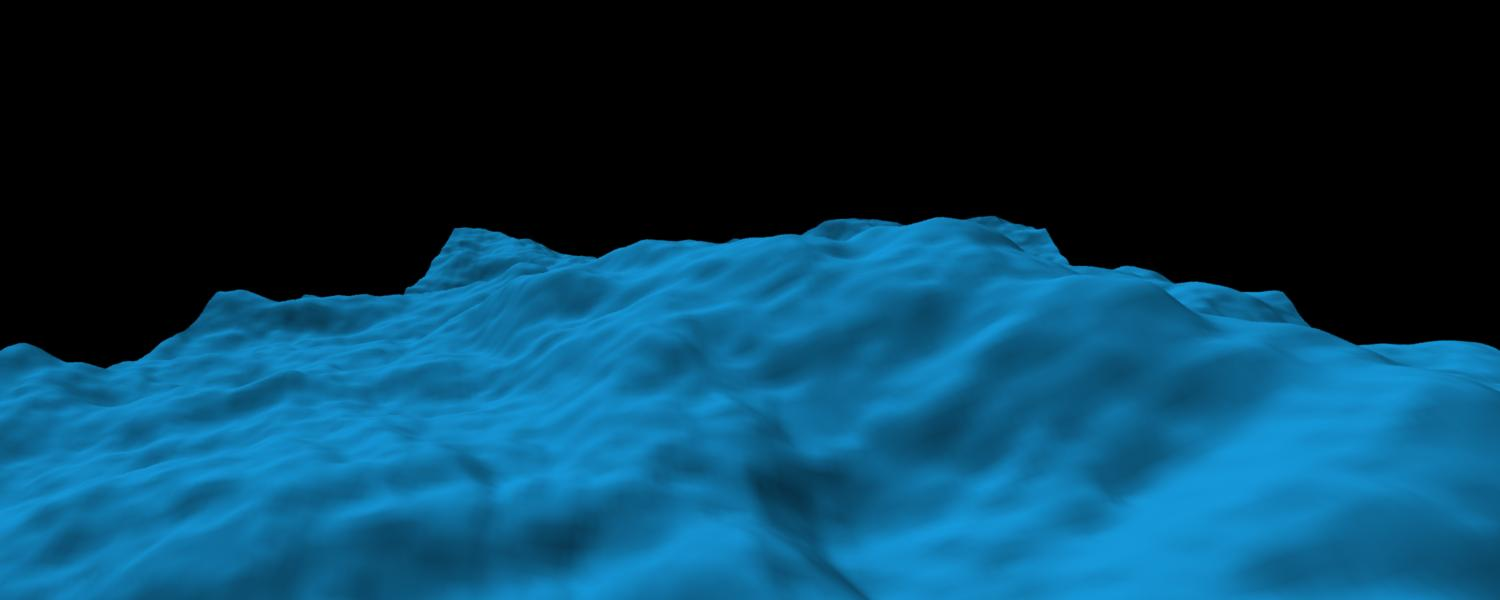
\includegraphics[scale=0.125]{figures/Simulating_Ocean_Water-012.png}
 }
 \subtop
 {
  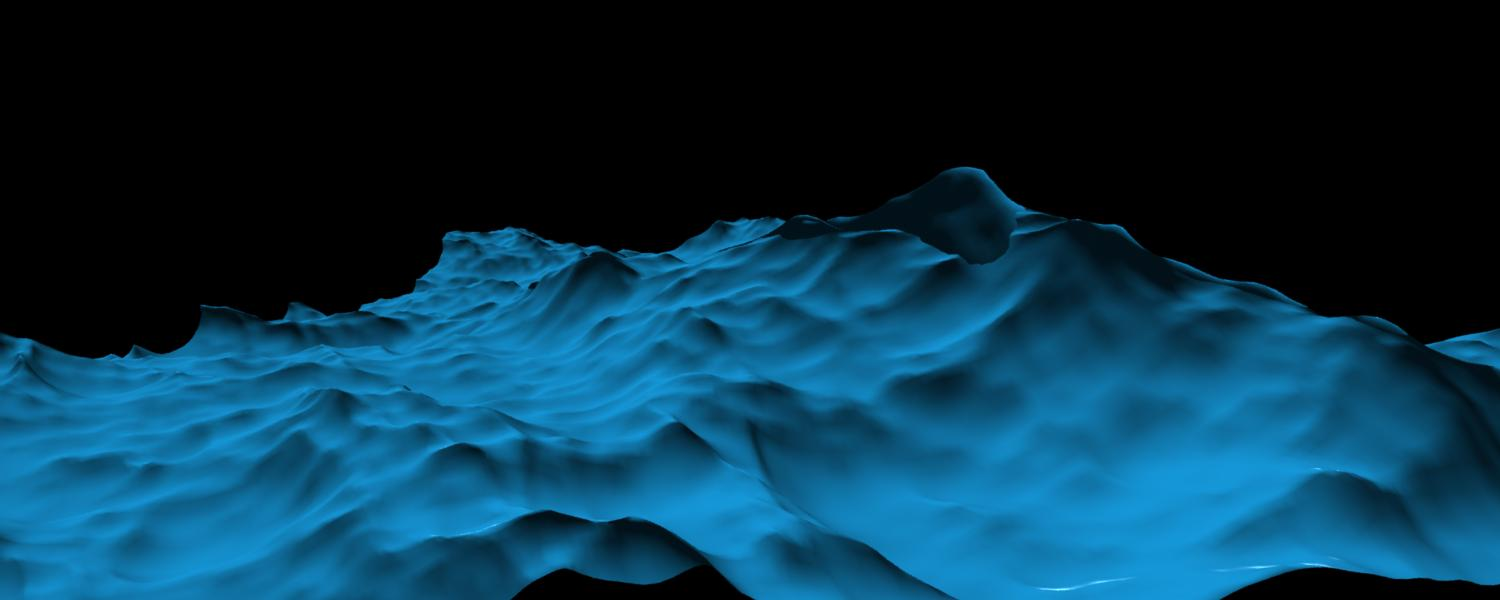
\includegraphics[scale=0.125]{figures/Simulating_Ocean_Water-013.png}
 }
 \caption{Tessendorf 1999}
\end{figure}

\begin{figure}
 \centering
 \subtop
 {
  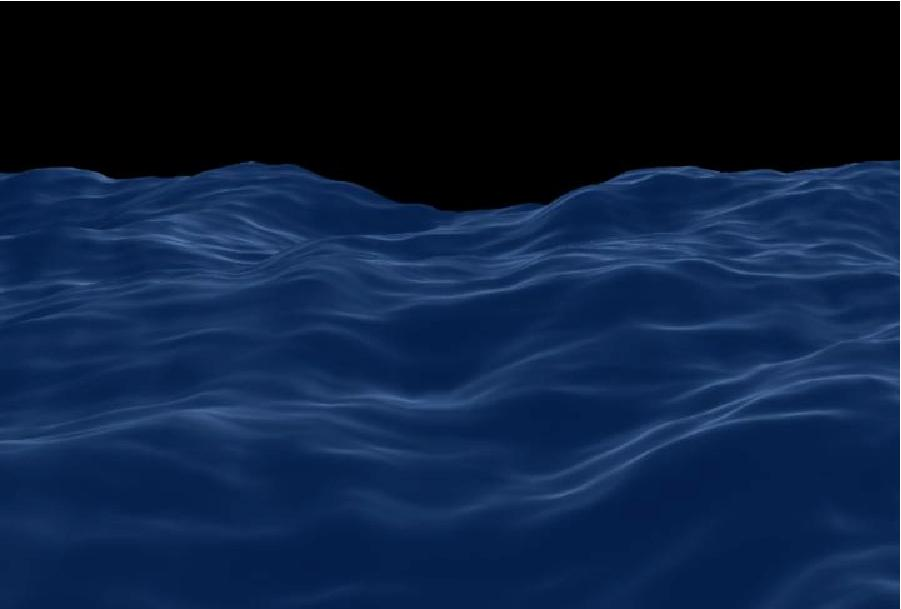
\includegraphics[scale=0.145]{figures/Simulating_Ocean_Water-008.png}
 }
 \hfill
 \subtop
 {
  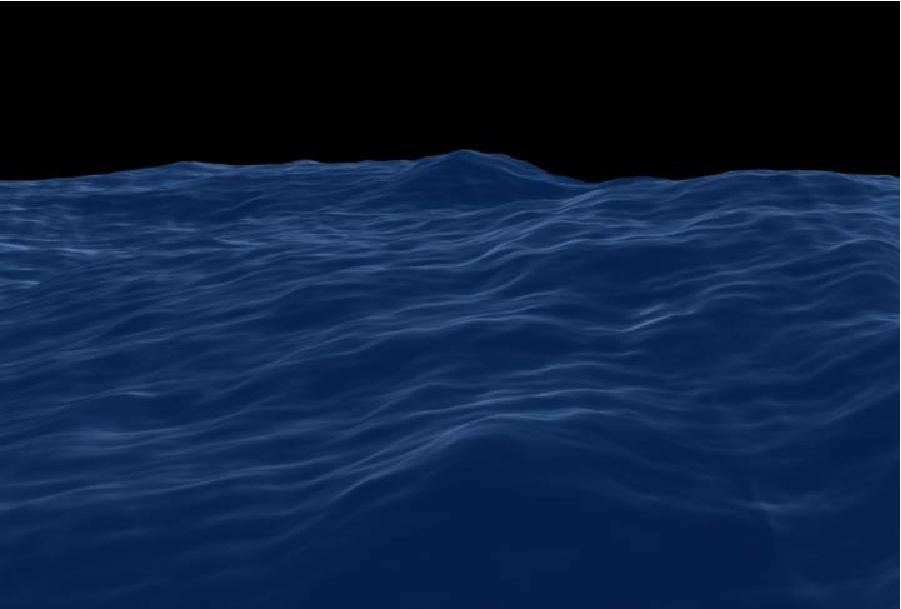
\includegraphics[scale=0.145]{figures/Simulating_Ocean_Water-009.png}
 }
 \hfill
 \subtop
 {
  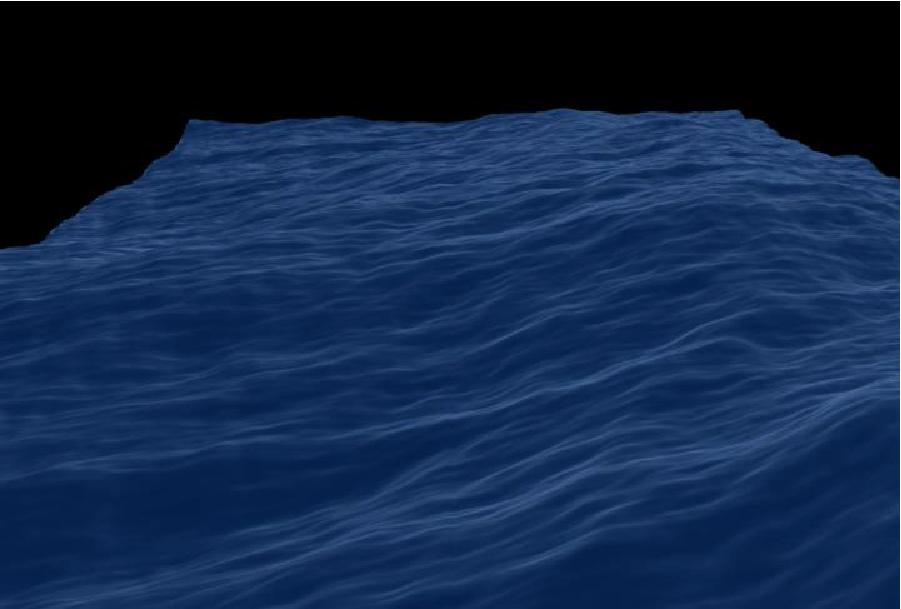
\includegraphics[scale=0.145]{figures/Simulating_Ocean_Water-010.png}
 }
 \caption{Tessendorf 1999}
\end{figure}